\documentclass[10pt,a4paper]{article}
\usepackage[UTF8]{ctex}
\usepackage{amsmath}
\usepackage{amsfonts}
\usepackage{amssymb}
\usepackage{float}
%\usepackage{clrscode}
\usepackage[]{algorithm2e}
\usepackage{graphicx}
% Set the margin of document.
\usepackage[top=10mm, bottom=12.5mm, left=12.5mm, right=12.5mm]{geometry}
\usepackage{longtable}
\usepackage{float}
\renewcommand\figurename{图}
\renewcommand\tablename{表}
\title{实验数据的插值}
\author{袁略真\\3130103964\\生物信息学\\浙江大学}
\begin{document}
\maketitle
\section{n次插值}
\subsection{插值的含义}
当两物理量x,y之间存在函数关系y=f(x),而其具体的函数关系式并不知道,为寻求其函数关系,常通过实验测得一组实验数据$x_0,...,x_n$及其对应的函数值$y_0,...,y_n$.插值根据这些对应关系,寻求函数f(x)的近似表达式,它常是x的多项式.插值满足的条件是:
\begin{enumerate}
\item 多项式的待定系数不超过数据个数
\item 多项式经过全部所给数据点
\end{enumerate}
\subsection{插值的应用场合}
\begin{enumerate}
\item 在已知数据具有高精度的情况下,甚至数据是通过推导绝对正确的情况下,获取给定数据点之外的函数取值.当已知值存在显著误差,则应考虑拟合.

\item 插值,如本堂课讲的用多项式进行插值,在计算上比较容易,计算结果又与目标函数值十分接近.

\item 有时,目标函数是已知的,如sin(x).计算机软件中它的值是通过多项式逼近来计算的\footnote{书$<$数值方法(MATLAB版)(第四版)$>$,(John H.Mathews, Kurtis D.Fink著)第4章.}.
\end{enumerate}

\subsection{使用n次拉格朗日多项式插值}
n 次插值多项式需要n+1个插值点.插值多项式和插值基函数由一下两式表示.
$$y(x)=\sum\limits_{j=0}^n A_j (x) y_j$$
$$A_j (x) = \prod\limits_{i=0,i\neq j}^n \frac{x-x_i}{x_j-x_i}$$

\section{程序流程}
\begin{algorithm}[H]
\KwIn{$x_0,\ x_n,\ n,\ file$}
\KwOut{a matrix of \textit{x},predicted value \textit{y},the real value \textit{yreal}}
\For{$i \gets 0$ \KwTo N}{
	calculate $x_i,y_i$,and store in the vector \textit{x}, and \textit{y}\;
}

\For{$x_t\gets x_0$ \KwTo $x_n$, sample 100 points}{
	$result \gets 0$\;
	\For{$j \gets 0$ \KwTo n}{
		$Aj \gets 1$\;
		\For{$i \gets 0$ \KwTo n}{
			\If{$i \neq j$}{
				Aj*=($x_t$-x[i])/(x[j]-x[i])\;
			}
		}
		result+=Aj*y[j]\;
	}
	print $x_t$,result,y(xt)\;
}
 \caption{拉格朗日插值法}
\end{algorithm}

\section{模拟及结果}
\subsection{模拟的参数设置}
固定x0=5,xn=95,file name = ``result".令n=2,4,6分别运行3轮.

\subsection{模拟的图形结果}
\begin{figure}[H]
\centering
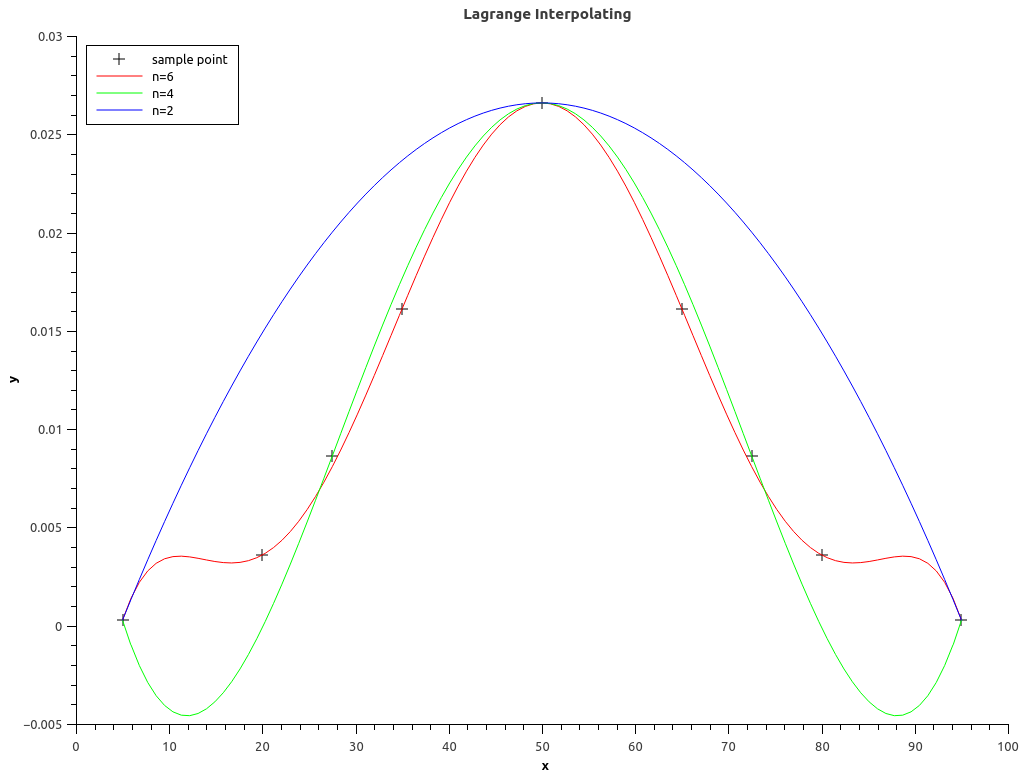
\includegraphics[width=0.6\textwidth]{../result/Graph2.png}
\caption{拉格朗日插值法分别在n=2,4,6下的插值曲线.其中目标函数是正态分布的概率密度函数,均值50.0,方差15.0.如图例所示,黑十字表示在3轮插值中先后出现的样本点,蓝色曲线表示仅有3样本点时抛物线型曲线,绿色、红色曲线则分别对应4、6个样本点时曲线.}
\end{figure}
\end{document}